\justifying
\NSFCBodyText

\subsubsection{研究内容}

本项目围绕“相近低质量表征为何形成不同作用路径与反事实响应”这一中心问题，将结构缺陷削减和非冗余语义支持损失拆分为两条可独立反证的路径。研究对象限定为许可可追溯的公开中文语料与小中规模开源自回归模型的继续预训练。主要结果由训练运行层面的路径效应、处理特异性、能力定向梯度对齐和独立来源复核共同判定，不以质量评分器的榜单性能或最优筛选阈值判定。

\paragraph{研究内容一：构建中文低质量表征“同分异源”的可识别样本层。}

选择两个彼此独立、许可和版本可核验的公开中文语料来源。来源 A 用于形成和检验假设，来源 B 仅在协议冻结后用于外部复核，并须具有足够的目标语体独立 token、独立站点/时间层和可执行的跨来源近邻去重；任一条件不满足时，来源 B 只复核仍满足准入条件的路径。对语料完成来源审计、隐私和敏感内容处理、文档级与跨文档去重、语言/编码检查及数据卡记录，按来源、主题/实体、语体与重复簇建立索引。正式语料名称将在许可与独立 token 审计后确定，暂定一个异质网页/社区来源与一个相对规范的百科或知识来源；若严格处理后任一关键臂无法提供共同训练预算所需的独立 token，则所有臂统一下调预算，不以重复曝光补足。

在中文现象上，预注册一类结构完整、来源可核验但模型低熟悉的中文语体作为确认性对象，暂定为规范书面表达与网络/地域书写语体的语义匹配对；另从简繁/异体或中英混写中选择一种作稳健性复核。对照定义不依赖“是否规范”的价值判断，而由四项可观测条件共同确定：结构与语义完整性经人工复核，来源可追溯，语料中出现频率较低，独立定位模型判断的处理前熟悉度较低。候选定位使用与确认性基座、诊断集和最终测试集隔离的数据分片与评分模型；确认性基座的处理前熟悉度只作为冻结协变量和效应调节量，不参与样本纳入。两名以上标注者在不知道质量分和实验结果的条件下判断结构完整、语义保持、事实一致与语体属性；一致性不足时先修订标注规范，不进入确认性训练。

质量表征至少包含两类异质信号：一类为独立定位模型给出的困惑度或可学习性连续分数，另一类为来源/规范性分类或多维质量分数\cite{zhuang2025metarater,bai2025multiactor,xu2025fire,ali2025jql}。质量分只用于定位结构破损样本与完整低熟悉语体的分数重叠区域，不作为因果暴露，也不读取确认性训练或能力结果。对两类样本进行分层匹配并报告分数、长度、来源、主题和 tokenization 的平衡情况；若“同分”只出现在一个评分器或无法达到预注册重叠标准，则中心“低质量表征效用异质性”命题判为不成立。此后两条干预至多作为结构损伤和支持广度的独立子研究，不再用于支持本项目题目所述中心结论。

研究内容一将形成可审计的数据卡、中文语体操作定义、人工标注规范、两类评分器版本、同分样本层和六个处理臂的确定性生成器。此阶段依据许可可追溯性、人工一致性、语义保持、评分重叠和处理臂平衡验收，不提前比较模型性能。通过验收的样本层用于后续两条路径的随机干预。

\begin{center}
\begingroup
\small
\renewcommand{\arraystretch}{1.12}
\begin{tabular}{p{0.08\textwidth}p{0.55\textwidth}p{0.27\textwidth}}
\hline
臂 & 唯一处理 & 所属对比 \\
\hline
A0 & 共同破损前体经精确逆操作恢复，保留目标语体 & 两条路径共同参考 \\
A1 & 保留共同前体的结构破损状态 & 结构损伤总效应 \\
A2 & 对共同破损前体作等量无效操作，不恢复结构 & 结构处理特异性 \\
A3 & 移除目标语体，补入等 token 主流文本 & 支持损失/伪补回 \\
A4 & 移除同一集合，补入同语体非冗余样本 & 支持补回主臂 \\
A5 & 移除同一集合，补入同语体窄支持样本 & 排除单纯语体曝光 \\
\hline
\end{tabular}
\endgroup
\end{center}

A0--A2 与 A3--A5 使用互不重叠的目标文档集合；各主对比共享背景池与训练预算，只改变表中所列处理。A0 中结构目标由共同破损前体经精确逆操作恢复，语体目标则保持原支持，是两条路径的共同参考；两个路径的估计量不作方向比较。

\paragraph{研究内容二：识别结构缺陷削减的训练效应、动力学证据及来源边界。}

针对段落错序、异常截断和连接结构破坏等可逆低层缺陷，从研究内容一的结构完整文档中随机生成共同破损前体。A1 保留该破损状态，A0 对前体实施精确逆操作恢复原结构，A2 对同一前体实施操作次数、位置与长度变化匹配但不恢复结构的 sham；A0 与 A2 经历相同次数的后续处理。优先选择能够保持核心语义单元、字符/token 长度与序列边界近似可比的操作；对无法配平的编辑记录其 tokenization、截断和 packing 差异，不据此作机制归因。三臂保持来源、主题、文档数、非 padding token、更新步数、优化器、数据顺序区组和总训练预算一致。

在来源 A 的同一初始 checkpoint 上，对三个处理臂进行成对随机继续预训练。训练运行是主推断单位，同一主种子成对控制语料抽样、batch 顺序、dropout 和评测随机性；token、checkpoint 和 benchmark 条目均不作为额外重复。结构路径的主要能力终点为预注册的通用语言与知识保持聚合指标，主要对比为“结构完整相对结构破损”的总效应，以及“结构完整相对 sham 编辑”的处理特异效应。能力结果揭盲前先完成结构标签、语义保持、tokenization 和 packing 的操纵验收；预期排序锁定为结构完整优于结构破损和 sham，且结构破损与 sham 落入预设等效区间。若 sham 与完整等效，首先判为操纵失败或当前剂量下结构效应不可识别，结构路径停止，不以优化器重调作事后挽救。

主动力学读出定义为“能力定向梯度对齐”：在确认性结果揭盲前固定的 checkpoint 和 probe mini-batch 上，对模型末层低秩投影梯度计算处理语料与完全独立能力诊断集之间的单位 token 归一化余弦；内积只作敏感性分析。主公式、投影维度、checkpoint 位置、probe 生成规则和归一化方式写入冻结分析清单，同一 manifest 只产生一个主读数。它表征局部更新对诊断目标的一步预期方向，不等同于完整因果中介。损失波动、梯度有效秩、裁剪率和遗忘率作为次级稳健性指标。只有当处理先改变主读出、主读出对独立后测能力有留出预测增益，并且原文恢复时读出与能力共同逆转，才认为结果支持动力学候选机制；任何一项失败均降低结论强度，不以次级指标替换主结果。

来源 A 上的分析完成后，冻结结构操纵、主终点、动力学读出、效应方向、预测区间和统计代码，在来源 B 上只复核 A0--A1 主对比，不重新选择阈值和指标。来源或操纵验收失败判为不可复核，区间过宽判为证据不足；只有条件均通过后效应仍反号或持续落在冻结区间之外、且一次固定预算校准无改善时，才拒绝该结构效应外推。研究内容二最终给出结构路径的运行级效应、恢复特异性、动力学证据及来源边界。

\paragraph{研究内容三：识别非冗余语义支持损失及其状态—来源—尺度边界。}

从研究内容一的确认性中文语体中固定一个待移除集合，在相同背景池和训练预算下构造四种状态：保留原语体支持的完整参考；移除目标语体后补入等 token、匹配长度与质量分的主流文本；移除同一集合后补入不重合、非冗余的同语体样本；移除同一集合后补入同语体等量重复或主题/实体高度集中的窄支持样本。目标语体内部的非冗余广度优先由来源、主题/实体分层和去重簇定义，嵌入覆盖指标只作辅助验证，避免用另一个黑箱分数重新定义“支持”。

支持路径先以 A0--A3 定义移除目标语体并以主流文本补回所产生的支持损失总效应，再用两个必要特异性对比解释该损失：A4--A3 判断同语体非冗余补回的恢复效应，A4--A5 排除“只要增加同语体 token 曝光即可”的替代解释。主要能力终点为目标语体与长尾能力聚合指标；完整路径还要求 A4 与 A0 落入预注册等效范围。若 A4 优于 A3、A5 但未与 A0 等效，只称部分恢复；若非冗余与窄支持均优于主流补回但二者无差异，结论收缩为语体曝光效应；若三者无差异，则支持路径不成立。

评价集与训练补回语料按文档、作者/站点、时间、主题和高阶表达模板隔离，并在不同词汇重叠阈值下重复分析，以排除直接记忆和评测对齐。能力定向梯度对齐在本内容中改用独立目标语体诊断集，检验同等语体曝光下非冗余支持是否形成更面向目标能力的更新。诊断集不兼作最终能力测试。

来源 A 上的支持路径通过后，一方面从同一基础训练轨迹的两个共同 checkpoint 随机分叉，检验“非冗余补回—窄支持补回”差异的状态调节；另一方面冻结 A4--A3 的处理规则、主终点、动力学读出、效应方向、预测区间和统计代码，在来源 B 上进行有限复核，不重新选择语体、阈值和指标。来源/操纵失败、区间过宽与条件通过后的真实异质分别报告，只有最后一类可触发拒绝外推。若两条路径在来源 B 均不保持方向，取消模型尺度探索；否则仅在同 tokenizer 家族的较大模型上复核少数关键臂。研究内容三最终给出支持恢复效应、语体曝光与非冗余广度的区分、动力学读出及状态—来源—尺度边界。

\subsubsection{研究目标}

总体目标是建立并检验中文预训练语料低质量表征效用异质性的双路径解释，获得结构缺陷削减与非冗余语义支持损失的路径特异证据、训练动力学候选机制及有限外部边界。

具体目标为：（1）形成可复核的中文“分数重叠、生成机制不同”样本层和反事实语料生成协议，区分结构完整性、模型熟悉度与静态质量评分；（2）估计结构修复相对破损与 sham 编辑的运行级效应，检验能力定向梯度读出的时间有序性、可恢复性及来源边界；（3）在语体曝光量匹配时区分同语体非冗余支持、同语体窄支持与主流文本补回，确定支持损失的动力学证据及状态、来源与尺度边界。

上述目标均不以“模型性能必须提升”为完成条件。若结构或支持路径被负对照否定，项目将按预注册规则删除相应机制，并报告可替代解释及其边界；这种可反证性本身是研究目标的组成部分。

\subsubsection{拟解决的关键科学问题}

\paragraph{结构缺陷路径。}在语义单元、来源、分词/packing 与训练预算匹配的可逆干预中，结构破损及其原文恢复如何改变能力定向梯度对齐；该读出是否构成通向独立通用能力变化的可重复候选中介？

\paragraph{非冗余支持路径及状态边界。}在低频中文语体 token 曝光量与静态质量匹配时，非冗余支持相对等量重复/窄支持是否产生特异的语体与长尾能力增益；该效应如何受共同 checkpoint 的处理前知识状态调节？

\paragraph{有限外部效度。}两条随机干预效应及其能力定向梯度读出中，哪些能在独立中文语料来源中复现，哪些只能在固定目标样本预算下校准；何种支持不足或不确定性应触发拒绝外推？

\subsubsection{研究方法与技术路线}

\paragraph{总体技术路线。}以两个可追溯的公开中文语料来源为输入，先由研究内容一构建“同分异源”样本层和六臂反事实语料；然后并行进入研究内容二的结构缺陷削减路径和研究内容三的非冗余语义支持路径。两条路径均先在来源 A 进行成对随机继续预训练和动力学检验，再将存活对比冻结后转入来源 B 复核，最终给出路径是否成立及其状态、来源和尺度边界。

总体流程为：来源审计与盲法标注 $\rightarrow$ 同分样本层与六臂语料 $\rightarrow$ 来源 A 双路径随机干预 $\rightarrow$ 能力与动力学联合判定 $\rightarrow$ 来源 B 冻结复核。

\begin{figure}[htbp]
  \centering
  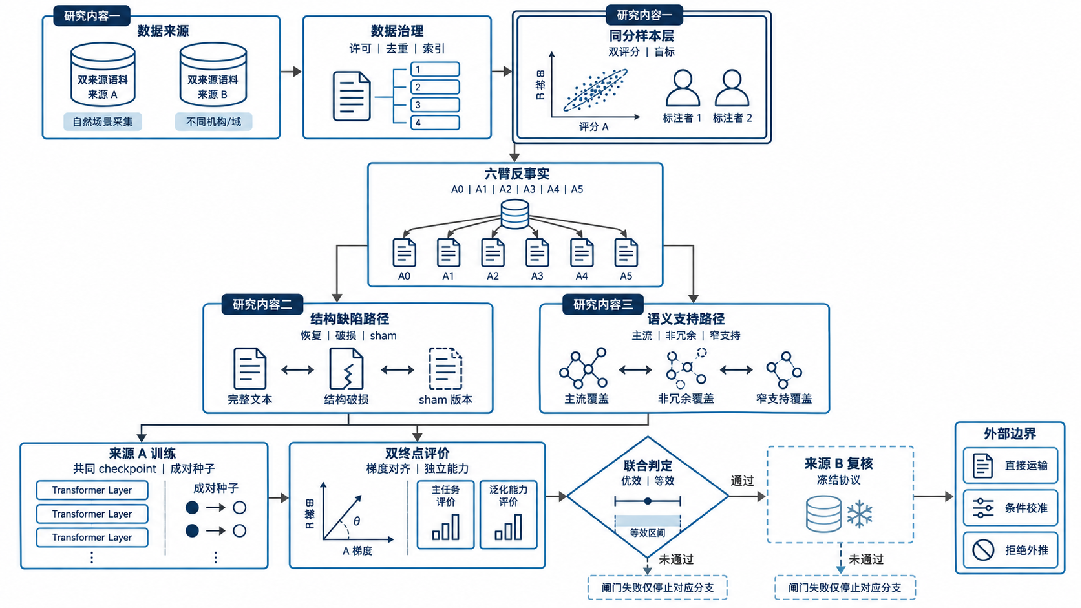
\includegraphics[width=0.98\linewidth]{figures/F03-overall-framework.pdf}
  \caption{三项研究内容与双路径证据闭环总体框架}
  \label{fig:overall-framework}
\end{figure}

\paragraph{共性训练、测量与统计方法。}研究内容二、三共用约 1B 规模开源基座，每个处理臂设六个成对主种子，匹配非 padding token、序列长度、优化器、更新步数与训练 FLOPs。单次训练暂定 0.40B token，实际值仅根据先导吞吐、独立语料规模和揭盲前功效模拟校准。训练运行 $r$ 是唯一主推断单位，checkpoint、batch 和 probe 文档不作为额外重复。

在 checkpoint $t$ 上，定义处理臂 $a$ 对能力 $k$ 的定向梯度对齐为
\begin{equation}
G_{rkt}^{(a)}=
\frac{\left\langle g_{\mathrm{train},rt}^{(a)},g_{\mathrm{probe},kt}\right\rangle}
{\left\lVert g_{\mathrm{train},rt}^{(a)}\right\rVert_2
 \left\lVert g_{\mathrm{probe},kt}\right\rVert_2},
\end{equation}
其中两类梯度都经单位 token 归一化并投影到预先固定的末层低秩子空间。仅当处理先改变 $G$、$G$ 对独立后测能力具有留出预测增益，并在恢复或支持补回时与能力共同逆转，才视为候选动力学证据。两条主路径各预分配单侧 $\alpha=0.025$，以六个配对区组的精确符号翻转检验和交并式联合规则作正式判定。训练、probe 与最终测试集分层隔离，所有运行由唯一 manifest 追踪。

\paragraph{研究内容一对应路线：同分异源样本层构建。}以两个公开中文来源为输入，完成许可、隐私、去重和来源审计，建立来源—语体—主题/实体—重复簇索引。以困惑度/可学习性和来源/规范性两类分数组成 $\mathbf{s}(x)$，将结构破损样本 $x_i^{\mathrm{dam}}$ 与完整低熟悉语体 $x_j^{\mathrm{lf}}$ 的可匹配集定义为
\begin{equation}
\mathcal{M}_{\varepsilon}=\left\{(i,j):
\left\lVert\widetilde{\mathbf{s}}(x_i^{\mathrm{dam}})-
\widetilde{\mathbf{s}}(x_j^{\mathrm{lf}})\right\rVert_{\infty}\leq\varepsilon,
\ B_{ij}=1\right\},
\end{equation}
其中 $B_{ij}$ 表示长度、来源、主题和 tokenization 已通过预注册平衡，$\varepsilon$ 在不读取能力结果时冻结。两名以上标注者盲法复核结构完整、语义保持、事实一致和语体属性，关键维度 Krippendorff $\alpha$ 低于试标后冻结的阈值则返工。

对 $\mathcal{M}_{\varepsilon}$ 中的样本分层匹配，以统一背景池生成 A0--A5，并审计独立 token、重复曝光、语体比例、主题覆盖、padding、截断和 FLOPs；主对比的有效 token 或 FLOPs 偏差暂定不超过 $2\%$。本路线输出数据卡、标注规范、同分样本层和确定性六臂生成器；许可、一致性、语义保持、分数重叠与臂间平衡均通过后，分别向研究内容二、三输出互不重叠的目标文档。

\begin{figure}[htbp]
  \centering
  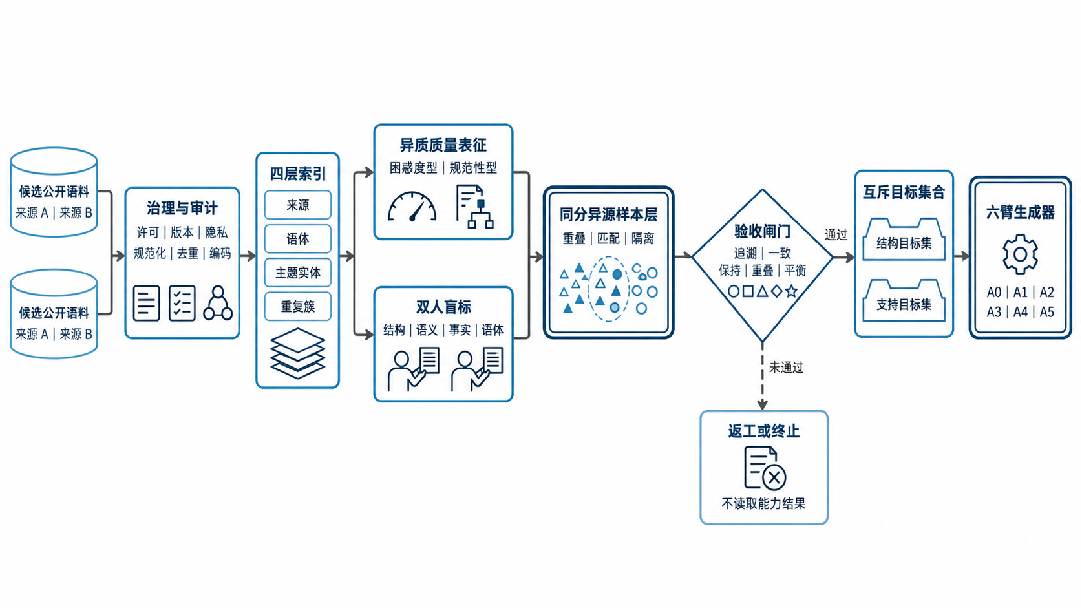
\includegraphics[width=0.98\linewidth]{figures/F04-route-1-sample-layer.pdf}
  \caption{研究路线一：同分异源样本层构建与验收}
  \label{fig:route-sample-layer}
\end{figure}

\paragraph{研究内容二对应路线：结构缺陷削减的效应、动力学与来源边界。}以研究内容一产出的结构完整文档和生成器为输入，建立共同破损前体：A1 保留段落错序、异常截断或连接破坏，A0 依索引精确恢复，A2 执行等量但无恢复作用的 sham。三臂通过 tokenization、packing、曝光量和训练预算验收后，从来源 A 的共同 checkpoint 成对继续预训练。对运行 $r$ 的通用能力终点 $Y_r(a)$，定义
\begin{equation}
\tau_{\mathrm{str}}=\mathrm{E}_{r}\!\left[Y_r(\mathrm{A0})-Y_r(\mathrm{A1})\right],\qquad
\tau_{\mathrm{spec}}=\mathrm{E}_{r}\!\left[Y_r(\mathrm{A0})-Y_r(\mathrm{A2})\right].
\end{equation}
$\tau_{\mathrm{str}}$ 估计结构恢复相对破损的总效应，$\tau_{\mathrm{spec}}$ 检验该效应是否超出等量编辑本身。

两个对比的单侧 $97.5\%$ 随机化反演置信下界均超过各自最小实践意义阈值，且 $G$ 满足时间先行、留出预测和恢复共同逆转时，才确认完整结构路径。随后冻结 A0--A1 的处理规则、方向、区间和代码，在来源 B 复核：准入/操纵失败判为不可复核，区间过宽判为证据不足，条件通过后仍反号或超出冻结区间才触发校准或拒绝外推。本路线输出结构效应、动力学证据及来源边界，路径失败则停止其外部复核。

\begin{figure}[htbp]
  \centering
  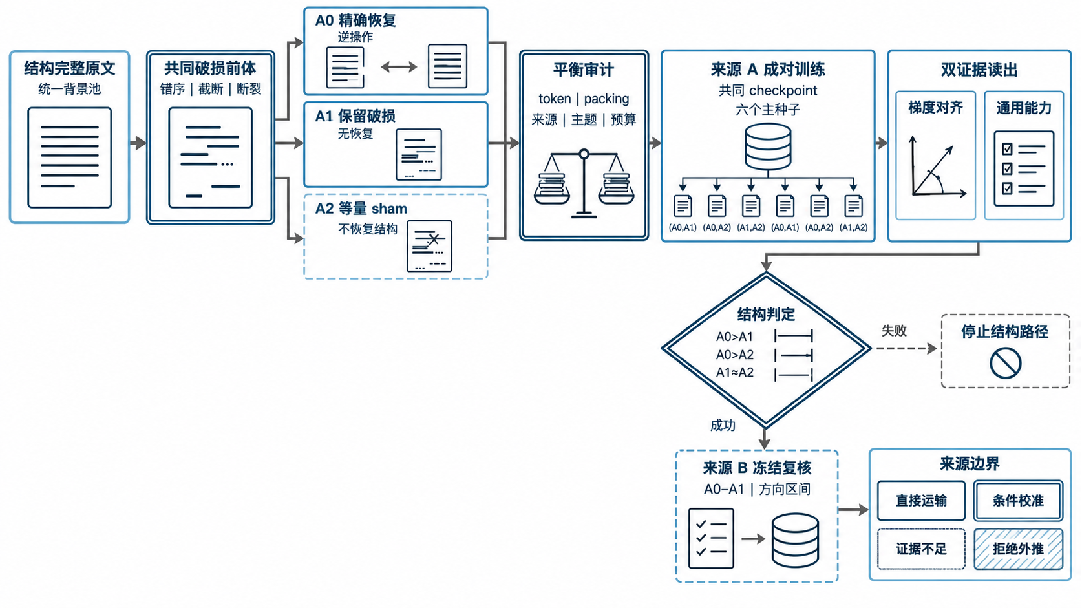
\includegraphics[width=0.98\linewidth]{figures/F05-route-2-structural.pdf}
  \caption{研究路线二：结构缺陷削减、动力学判定与来源边界}
  \label{fig:route-structural}
\end{figure}

\paragraph{研究内容三对应路线：非冗余语义支持的效应、动力学与状态—来源—尺度边界。}以研究内容一确认的目标语体、主题/实体层与去重簇为输入，固定同一待移除集合：A0 保留完整支持，A3 以等 token 主流文本补回，A4 以同语体非冗余样本补回，A5 以同语体窄支持补回。四臂通过语体曝光量、长度、质量分、tokenization、packing 和预算平衡后成对继续预训练。以目标语体/长尾能力 $Z_r(a)$ 为终点，定义
\begin{align}
\tau_{\mathrm{loss}}&=\mathrm{E}_{r}[Z_r(\mathrm{A0})-Z_r(\mathrm{A3})],\\
\tau_{\mathrm{restore}}&=\mathrm{E}_{r}[Z_r(\mathrm{A4})-Z_r(\mathrm{A3})],\quad
\tau_{\mathrm{breadth}}=\mathrm{E}_{r}[Z_r(\mathrm{A4})-Z_r(\mathrm{A5})].
\end{align}
三个效应分别表征支持损失、非冗余补回和超出单纯语体曝光的支持广度效应。完整恢复还需满足
\begin{equation}
\mathrm{CI}_{95\%}\!\left(\mathrm{E}_{r}[Z_r(\mathrm{A4})-Z_r(\mathrm{A0})]\right)
\subset[-\Delta_{\mathrm{eq}},\Delta_{\mathrm{eq}}],
\end{equation}
其中 $\Delta_{\mathrm{eq}}$ 由 benchmark 重测误差与科学最小意义在揭盲前冻结。

三个优效对比的单侧 $97.5\%$ 置信下界均超过阈值，且上述等效条件成立时，才确认完整支持路径；A4 未与 A0 等效时只称部分恢复，A4 与 A5 无差异时收缩为语体曝光效应。主路径通过后，从两个共同 checkpoint 分叉检验状态调节，并将 A4--A3 冻结后转入来源 B 复核；复核采用与研究内容二相同的准入、证据不足与拒绝外推规则。本路线输出支持效应、动力学读出及状态—来源—尺度边界；仅在至少一条路径于来源 B 保持方向时，才在同 tokenizer 家族较大模型上进行少量复核。

\begin{figure}[htbp]
  \centering
  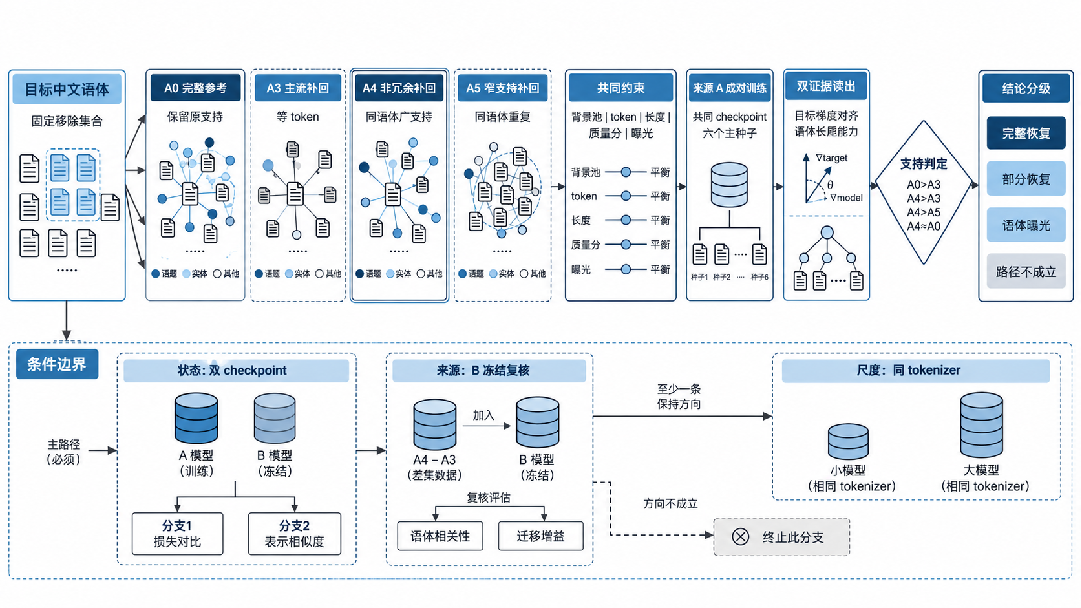
\includegraphics[width=0.98\linewidth]{figures/F06-route-3-semantic-support.pdf}
  \caption{研究路线三：非冗余语义支持及状态—来源—尺度边界}
  \label{fig:route-semantic-support}
\end{figure}

\subsubsection{关键技术}

\paragraph{结构与语义支持的可分离干预。}关键不是生成更多清洗版本，而是在保持语义支持时改变结构缺陷、在保持语体曝光时改变非冗余广度。需建立可逆结构编辑、等编辑量 sham、主题/实体分层补回和重复簇控制，使每个主对比只改变预定路径；无法达到预注册平衡时主动放弃强因果措辞。

\paragraph{能力定向梯度读出的低成本测量。}全数据、全参数影响函数不适合本项目资源。拟在固定的少量 checkpoint、probe 文档和末层/低秩梯度投影上计算目标定向对齐，统一单位 token 归一化和诊断集隔离；通过留一种子、留一来源预测与恢复共同逆转检验其有效性，控制计算与存储开销。

\paragraph{运行级可重复与泄漏防控。}所有科学运行由唯一 manifest 登记数据版本、处理臂、种子、token、优化配置、checkpoint 和评价版本；统计代码禁止把 checkpoint、题目或文档当作独立复制。训练、诊断和测试按多层近邻关系隔离，避免同语体恢复被直接记忆解释。来源 B 严格沿用来源 A 确定的协议，以降低外部验证中的二次调参偏差。

\subsubsection{可行性分析}

\paragraph{理论与方法可行。}数据筛选、多维评分、领域重加权与影响估计已形成可用方法基础\cite{harnessingdiversityfor2024,doremioptimizingdata2023,dogedomainreweighting2023,trainingdatainfluence2024,scalableinfluenceand2024}。本项目不需发明全新的通用预训练框架，而是把成熟的语料处理与梯度观测工具置于可逆干预和负对照中，用更严格的识别问题约束方法选择。主假设可由六个处理臂和两个能力终点直接支持或否定，统计层级明确。

\paragraph{数据与合规可行。}研究只纳入许可、来源和版本可核验的公开中文语料，先完成数据卡和可公开范围审计再训练。确认性语体只选一类，另一类作复核，避免现象清单膨胀。若目标语体不足以支持预定独立 token，则统一降低所有臂预算或收缩为较小代理模型，不重复曝光稀缺语料以制造样本量。

\paragraph{计算条件可行。}申请人团队现有稳定可用计算条件包括 A40 GPU 8 张和 RTX 3090 Ti GPU 6 张。处理 token 上限拆分为：首年六臂工程先导 $6\times0.10=0.6$B，来源 A 确认性训练 $36\times0.40=14.4$B，来源 B 冻结主对比复核 $24\times0.40=9.6$B，可选状态和尺度探索至多 2.8B，合计约 27.4B；其中可选 2.8B 在闸门失败或资源不足时取消。首年另以不超过 10M token 的 smoke test 实测吞吐、显存、I/O、checkpoint/probe 存储和评测成本，换算 GPU 时及失败重跑余量后再冻结年度运行矩阵；不把尚未落实的 A100 条件计入方案。

\paragraph{组织与风险可控。}数据许可、标注、训练、统计和泄漏审计之间有清晰接口，团队可按职责分工并用统一 manifest 汇总。停止规则预先覆盖操纵失败、路径无效和外部反号：评分重叠失败时，结论限于评分器的条件失配；sham 操纵不合格时停止结构路径，不报告处理特异结论；非冗余与窄支持无差异时，只保留语体曝光解释；动力学读出失败时，保留随机化总效应并删除候选机制解释；来源 B 的来源/操纵失败、估计不精确和真实异质分别报告。分阶段规则避免因单个环节失败而扩大实验搜索范围。
